\section{Load Balancer Parametrization}
% with graphics 2 pages -> with graphics got 5-6 pages.
With this range of experiments we set out to better understand the effects different parameters have on a load balancers performance.
We then continue to use this information to make an informed decision for the load balancer parameters in subsequent experiments.

Specifically, we want to understand the relationship between the following load balancer parameters:
\begin{enumerate}
    \item \textbf{Scaling Factor:} the factor which determines how linearly observed node performance is mapped to weights
    \item \textbf{Weight Range:} the size of the weight range the load balancer can use
    \item \textbf{Current Weight Reset:} whether or not it makes sense to reset the current weights of the load balancers when the weights are changed
\end{enumerate}

\subsection{Setup}

Since previous experiments have shown that the impact parameter changes can have are at times hard to predict, we decided to perform this evaluation using a grid-search, meaning that we rely on trying a large number of permutations to find patterns in their behaviour.
To test these settings we do not rely on the full FaaS-Sim environment, but rather perform isolated tests with a single load balancer and less sophisticated function and network simulations.

Since we are trying to evaluate how well load balancers choose upstreams, the upstreams are the comparatively most accurately simulated component.
The performance model of our simulated upstreams is closely informed by our notion of a node's performance level and capacity, which we outlined in our load balancing approach.
Thus, each simulated upstream has a set level of performance, which determines how long it takes for a request to be processed.
Since our aim is to keep this simulation simple, we consider the response time determined by the upstream to represent both the network and the \gls{fet} that would be observed in a real serverless system.
Each upstream samples its response times from a set of two lognormal distribution, one of which represents the \gls{fet}, while the other represents the network time.
To simulate the effect of high load, each upstream also has a set capacity, measured in requests per second.
If an upstream receives more requests per second than is has capacity for, \glspl{fet} start to degrade linearly, meaning that response times get longer in proportion to how overloaded the upstream is.

To represent different system conditions we introduce \textit{performance spread} as an input variable to these experiments that determines the how heterogeneous the performance of the simulated upstreams is.
The assumed system scenario is closely aligned with the one of our initial evaluation.
Relative to the load balancer a node can fall into one of four location categories, which determine the network distance from the load balancer: \textit{local}, \textit{city}, \textit{nation}, and \textit{global}.
Like it would  be in a real scenario, the probabilities of nodes falling into each of the categories gets progressively higher, meaning that a very low number of nodes will be local, while the majority will be \textit{global} and thus rather far away form a network perspective.
Apart from their location, nodes can fall into three performance categories, which are \textit{small}, \textit{medium}, and \textit{large}.
This performance category determines both the typical \gls{fet} of that node and its capacity.
Small and medium nodes are more likely to be located close to the load balancer, while large nodes are likely to be farther away in the network.
This is done to represent a typical edge computing scenario where relatively weaker compute is available locally, with a large amount available farther away, e.g. in the cloud.
The performance spread then determines how big the differences between the different categories nodes can fall into are.
A performance spread of 15 for example would correspond to as scenario where \glspl{fet} range from 10ms to 150ms, capacities from 5\gls{rps} to 100\gls{rps}, and network times from 5ms to 250ms.
A higher performance spread would indicate higher performance differences, while a lower one would indicate lower differences, with a performance spread of 1 indicating complete homogeneity.


To make an informed decision on load balancer parametrization we performed three experiments.
\subsubsection{Scaling Factor and Performance Spread}
In this evaluation we examine the effect the scaling factor has on performance in a variety of different scenarios.
To this end we tested scaling factors from 0,1 to 10.
Scenarios included performance spreads from 1 to 46, and all scenarios were repeated three times with request loads of 50\gls{rps}, 250\gls{rps}, and 1000\gls{rps}.
The weight range upstreams were mapped onto in this experiment is [1;10].
The experiment covers a simulated time frame of 1000 seconds.

\begin{figure}
    \centering
    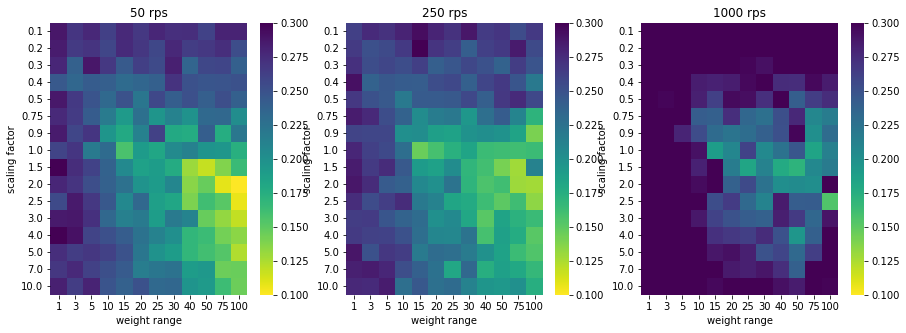
\includegraphics[width=14cm]{graphics/graphs/lb_hyper_scaling_vs_performance_spread.png}
    \caption{Mean response time over various levels of performance spread and scaling factors}
    \label{fig:lb_hyper_scaling_perfspread}
\end{figure}

The results of this experiment can be seen in Figure \ref{fig:lb_hyper_scaling_perfspread}.
Aside from showing lower performance for higher performance spreads, which is entirely to be expected since a larger performance spread means nodes are farther away and have higher \glspl{fet}, there are no significant differences between the scaling factors.

\subsubsection{Scaling Factor and Weight Range}
Analogously, we also evaluated the relationship between the scaling factor and weight range using a grid-search type experiment.
We once again tested scaling factors in the range [0,1;10] with request loads of 50\gls{rps}, 250\gls{rps}, and 1000\gls{rps}.
For the weight range the minimum weight was always set to 1, and the max weight between 1 and 100.
The performance spread was fixed over all experiments at 15, and the simulation is again run for 1000 seconds.

\begin{figure}
    \centering
    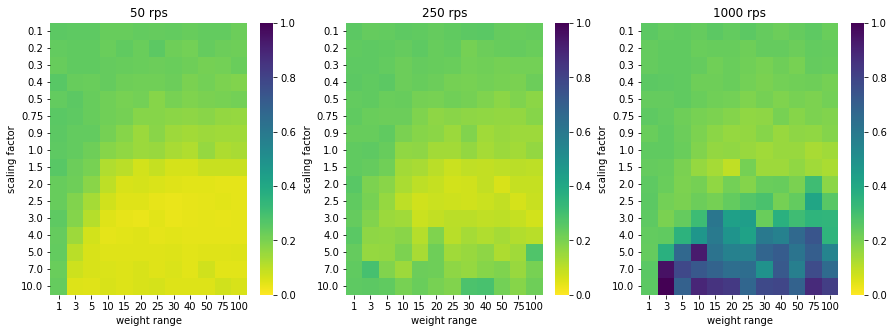
\includegraphics[width=14cm]{graphics/graphs/lb_hyper_scaling_vs_weight_range.png}
    \caption{Mean response time over different weight ranges and scaling factors}
    \label{fig:lb_hyper_weightrange_scaling}
\end{figure}

The results of this evaluation can be seen in Figure \ref{fig:lb_hyper_weightrange_scaling}.
Results show a clear trend towards higher weight ranges and scaling factors that are close to or slightly above 1, which would correspond to linear scaling.
We can also observe that higher request loads lead to worse performance on average, as one would expect, and also seem to shrink the set of configurations that provide good performance.

\subsubsection{Resetting Weights on Updates and Weight Update Intervals}
Our implementation of weighted round robin described earlier has a set of two weights for each upstream: the weight, and the current weight.
Once the weight of an upstream changes, we can choose to also reset the current weight or leave it as is.
Since intuitively there was no clear answer as to which choice is better, and the testing infrastructure around this was already in place, we chose to perform an experiment to measure the impact of this choice.
Apart from whether or not weights should be reset on updates, one also needs to decide at which interval weight updates should occur.
To evaluate this choice we performed these experiments using a variety of different update intervals.
Since we expected that resetting weights will have an outsized effect for scenarios with a low request rate, we performed experiments over a wider range of request loads than before, and also tested over different weight ranges.
Request load ranges from 2\gls{rps} to 1000\gls{rps}, weight update frequency from 5 seconds to 200 seconds, and maximum weight once again from 1 to 100.
Lastly, all experiments simulated a timeframe of 1000 seconds.

\begin{figure}
    \centering
    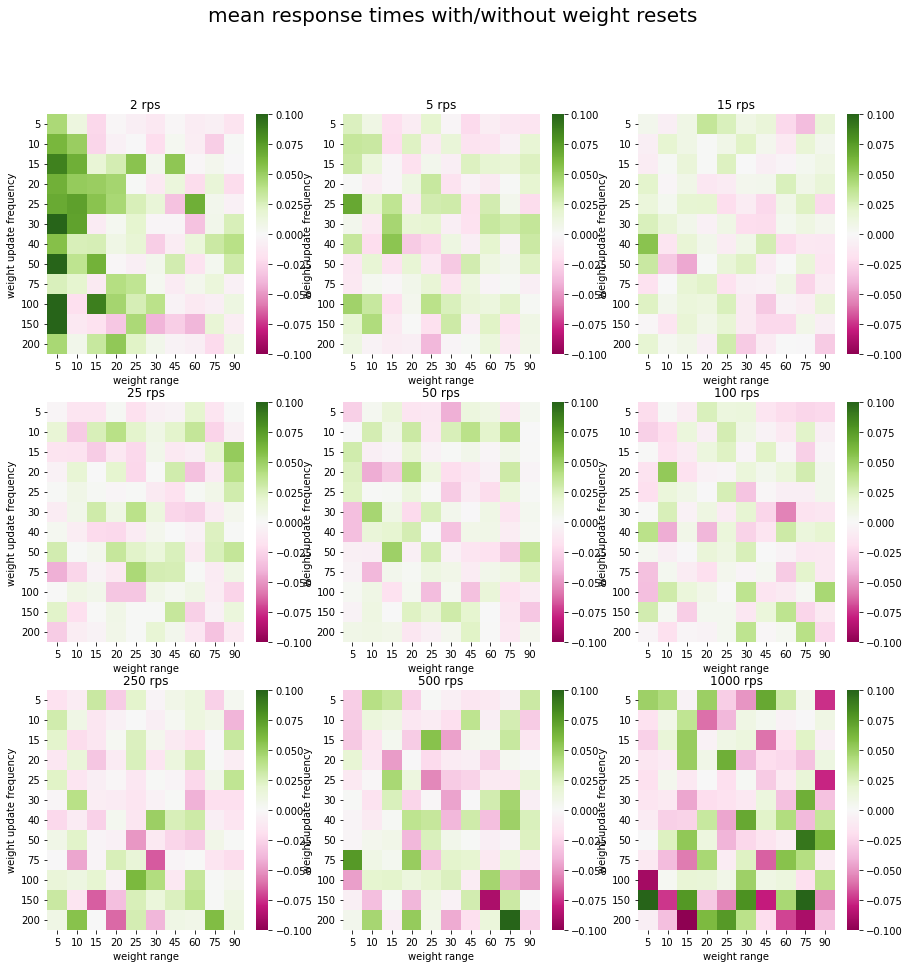
\includegraphics[width=14cm]{graphics/graphs/lb_hyper_weight_reset_delta.png}
    \caption{Difference between resetting and not resetting weights on update. Positive values indicate not resetting performs better, while negative values indicate the opposite.}
    \label{fig:lb_hyper_reset_delta}
\end{figure}

\begin{figure}
    \centering
    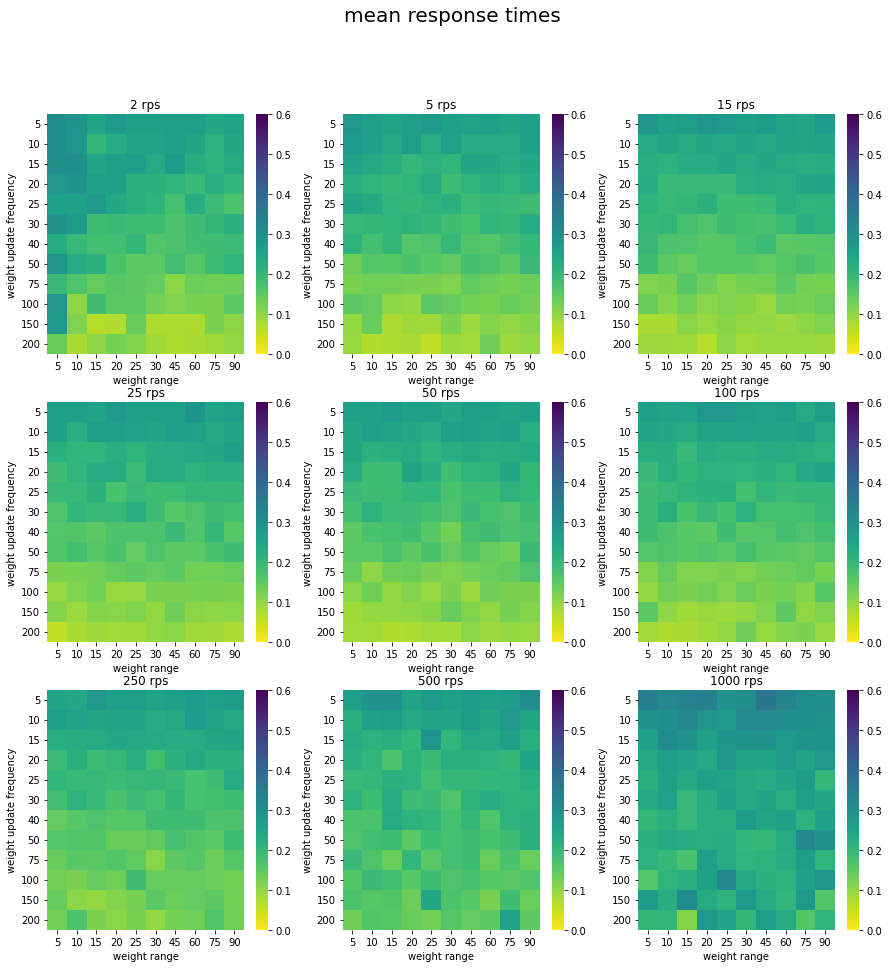
\includegraphics[width=14cm]{graphics/graphs/lb_hyper_mean_with_reset.png}
    \caption{Mean response times over different weight ranges and weight update times. Current weights are reset on update.}
    \label{fig:lb_hyper_reset_mean}
\end{figure}

\begin{figure}
    \centering
    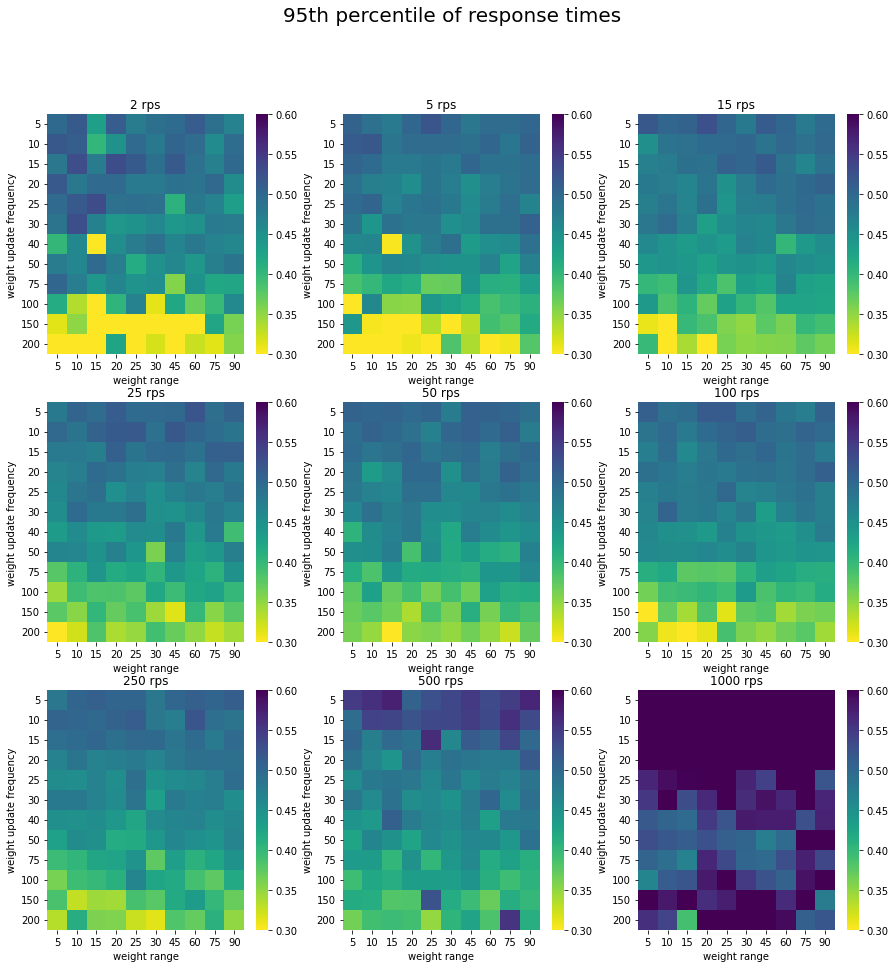
\includegraphics[width=14cm]{graphics/graphs/lb_hyper_95th_percentile_with_reset.png}
    \caption{95th percentile of response times over different weight ranges and update times. Current weights are reset on update.}
    \label{fig:lb_hyper_reset_q95}
\end{figure}

Figure \ref{fig:lb_hyper_reset_delta} shows the difference between the mean values of resetting or not resetting current weights.
In the results there is no clear indication resetting or not resetting is clearly superior.
There is a slight trend for not resetting performing better with low request rates, and resetting leading to better results in very high \gls{rps} scenarios.

Figure \ref{fig:lb_hyper_reset_mean} shows a trend towards longer intervals for weight updates performing better, irrespective of the weight range.
Figure \ref{fig:lb_hyper_reset_q95}, which shows the 95th percentile of the same data generally indicates the same tendency, although not for all request levels.
While at low request rates long update intervals perform better, they perform worse than shorter update intervals for high request rates.
Lastly we advise that care should be taken when comparing these visualizations, as the scale sometimes differs.
This is always indicated on the side of the visualization, and was necessary to better show relative differences within the same experiment run.


% Notes for discussion:
% QoS issue where one setting might be good under certain conditions, but bad under others e.g. 95th percentile type stuff
% extremes seem not to do so well for the most part
% behavious is to a large degree as expected: for low RPS super steep scaling works fine, but it becomes less good once capacity of the best nodes is reached
% No super clear point for or against weight resetting, once again depends on situation -> this points to a further investigation of the role of node discovery.
% to a degree weight resets perform a bit as expected in that low rps strongly prefer not resetting, and high rps preferring resets
% explanation why is quite intuitive, especially w.r.t. 